\capitulo{3}{Conceptos teóricos}
\section{Conceptos teóricos básicos}
Para facilitar la comprensión del proyecto, he seleccionado una serie de conceptos útiles a definir. 
\begin{itemize}
    \item Dinamómetro: artefacto destinado a la medición de la fuerza y el peso de los objetos a partir de la elasticidad de un resorte o muelle elástico.[Significados,s.f]
    \item Inclinómetro:
    \item Terapia ocupacional: 

\end{itemize}

\section{Estado del arte.}

Para iniciar el desarrollo del proyecto, se realizó una búsqueda del panorama actual en la medida de fuerza. 

En esta subsección se analiza y sintetiza el conocimiento existente en el área específica del proyecto. El objetivo principal es situar el trabajo dentro de un marco teórico y tecnológico, analizando investigaciones previas, aportes y detectar problemas que se puedan resolver.
\subsection{Dinamómetros:}
En la actualidad, los dinamómetros son una de las herramientas más utilizadas  para la medida de fuerza de los pacientes durante las sesiones de terapia ocupacional, fisioterapia o medicina deportiva. Existen diferentes modelos que varían en precisión, tecnología, precio o aplicación. 
A continuación, he destacado algunos de ellos:
\begin{itemize}
    \item Activforce 2: Es un dispositivo portátil e inalámbrico creado por la empresa estadounidense Activforce, con sede en California. Combina un dinamómetro con un inclinómetro lo que permite medir la fuerza máxima,promedio, rango de movimiento y simetría derecha-izquierda tanto en fuerza como en movimiento.Todas las mediciones se registran en una aplicación compatible con Android e iOS, donde el usuario puede ver toda la información recabada por el dispositivo. En la \textit{Figura 3.1} se puede ver una imagen del producto.
    \begin{figure}[h]
        \centering
        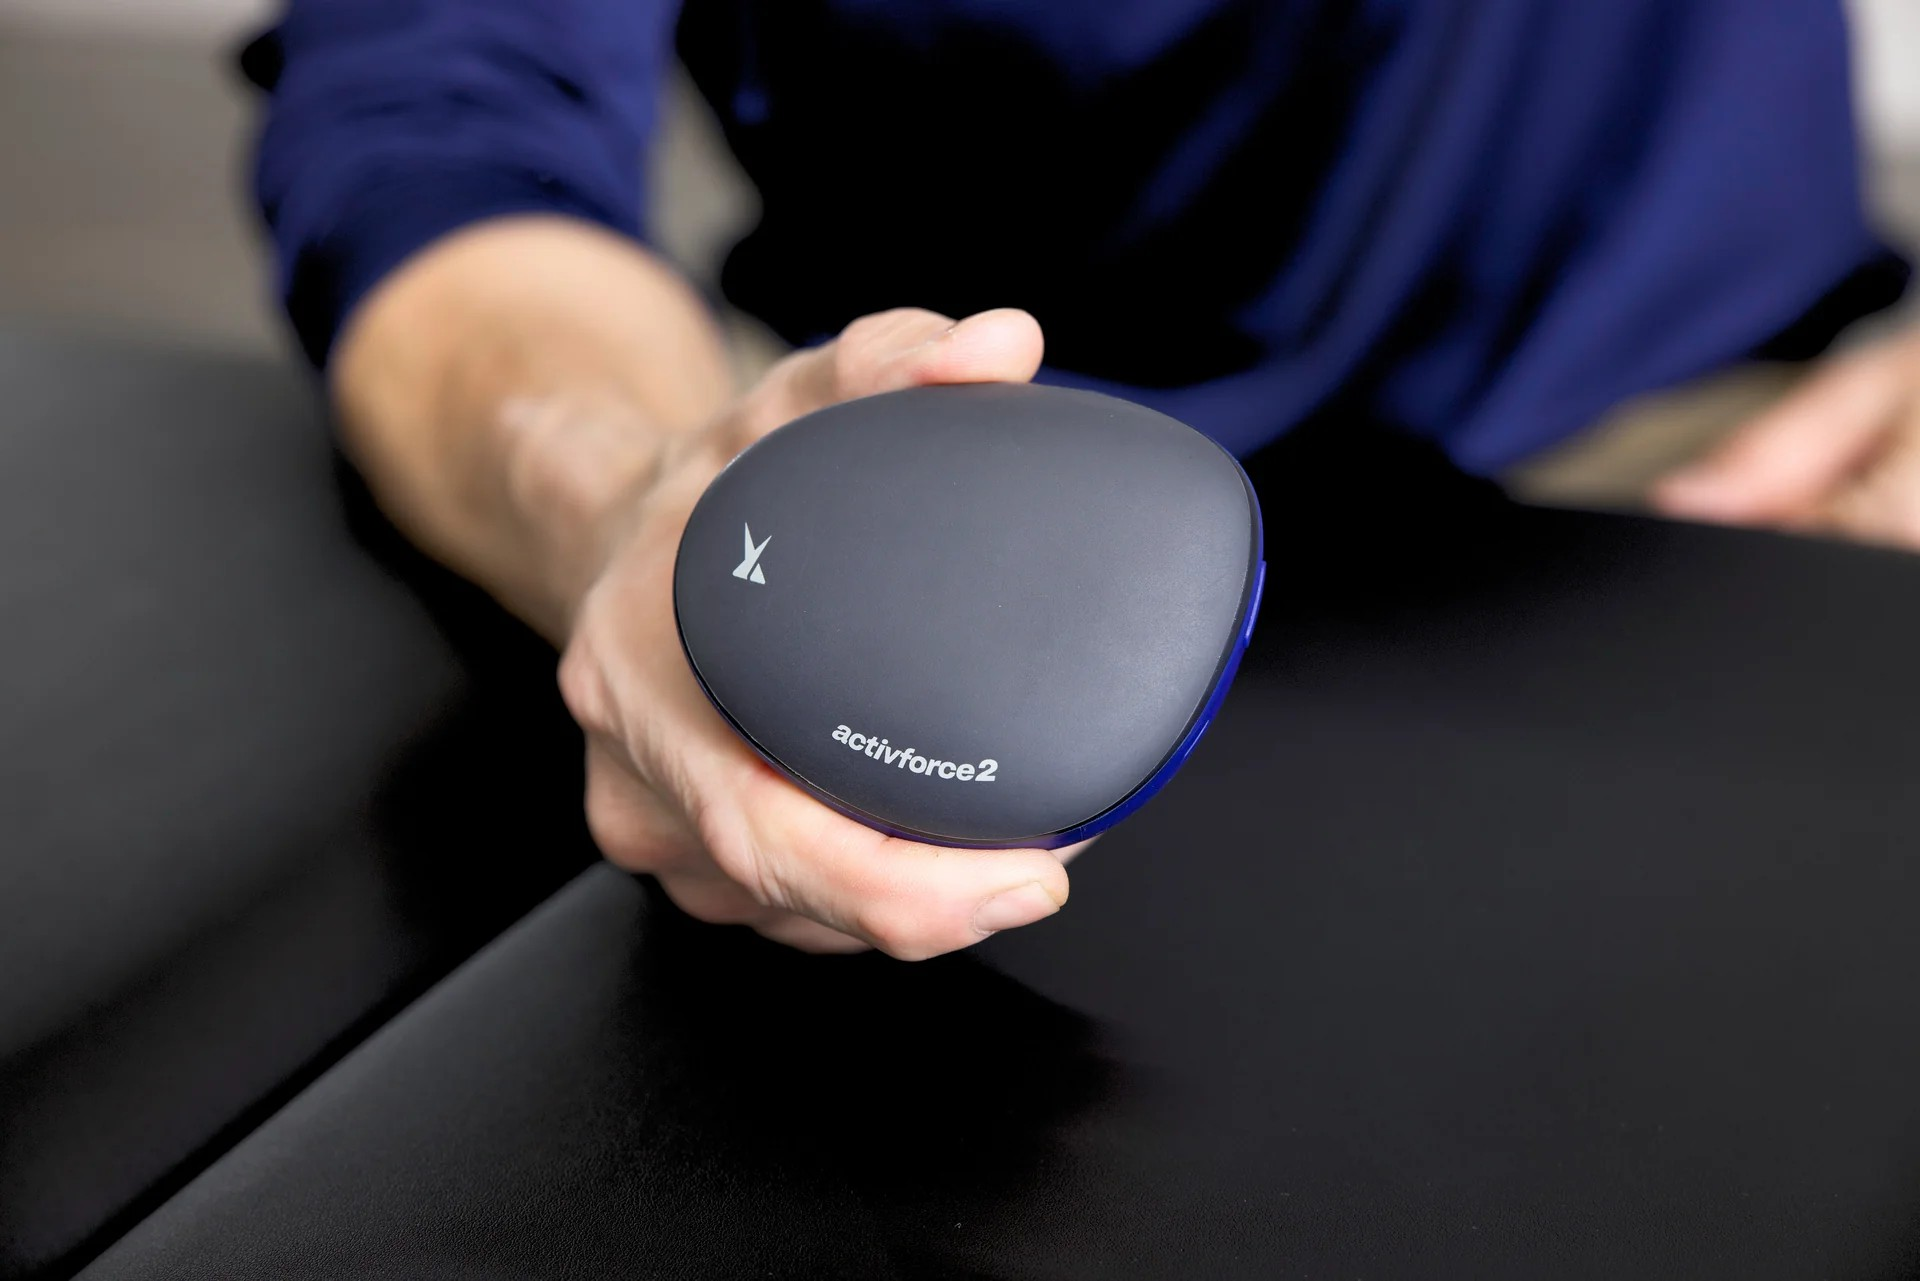
\includegraphics[width=0.5\textwidth]{img/ActivForce_Device.jpg}
        \caption{Dispositivo ActivForce2}
        \label{fig:activforce}
    \end{figure}
    
    Además, el Activforce 2 incluye varios accesorios que facilitan su uso en diferentes partes del cuerpo, permitiendo la ejecución de una amplia variedad de ejercicios y evaluaciones. Es un dispositivo de compra libre cuyo precio ronda los 450€. En la \textit{Figura 3.2} se puede ver una imagen del producto y los accesorios.
    \begin{figure}[h]
        \centering
        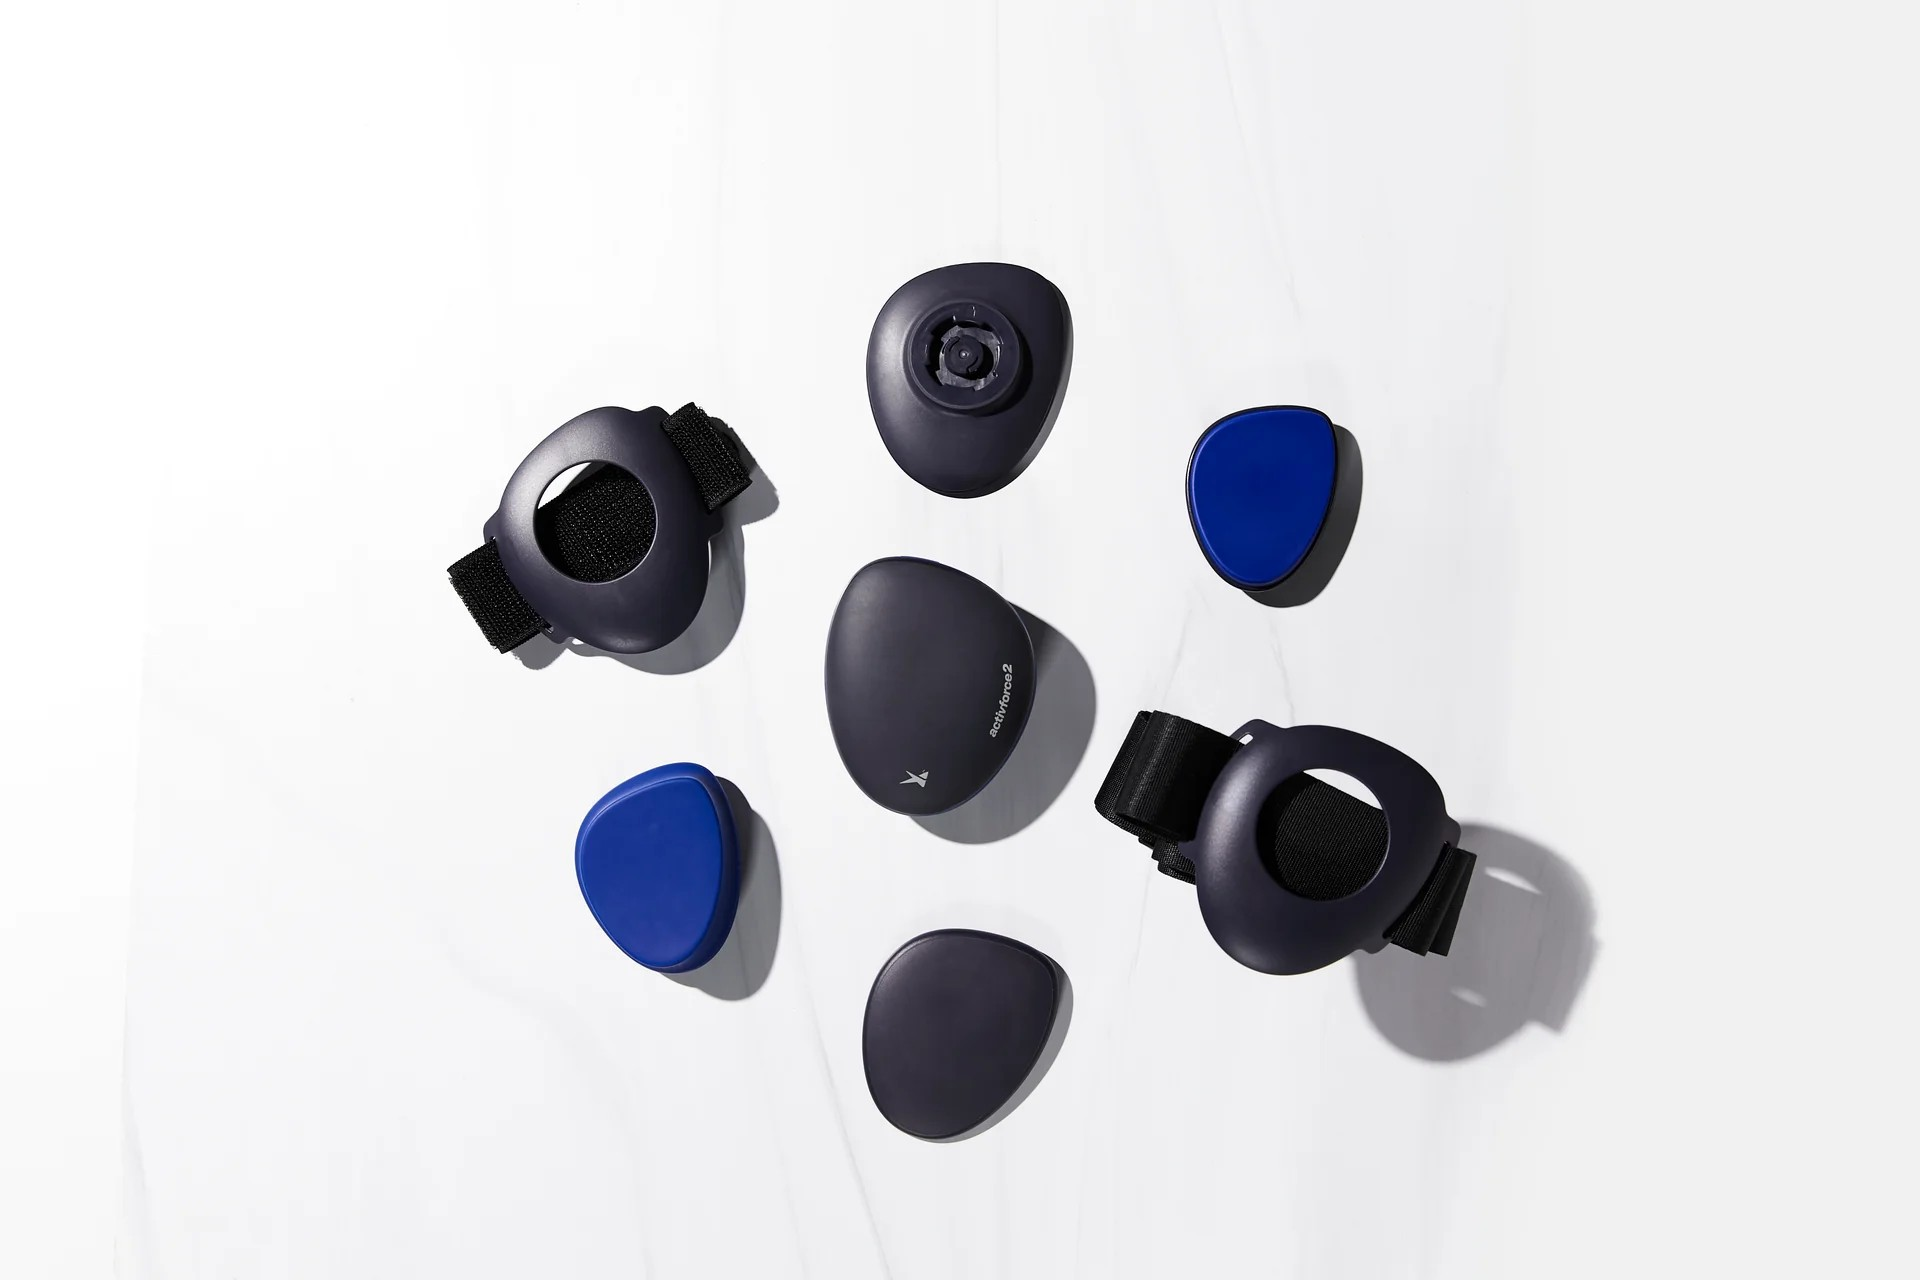
\includegraphics[width=0.5\textwidth]{img/ActivForce_Attachments.jpg}
        \caption{Accesorios compatibles con el dispositivo ActivForce2}
        \label{fig:activforce}
    \end{figure}

    \item MicroFET 2:Es un dispositivo portátil e inalámbrico creado por la empresa belga MVS in motion. Es un dinamómetro diseñado para la evaluación y prueba de fuerza permite tomar mediciones de prueba muscular objetivas, cuantificables y confiables.
    Es utilizado para la ayuda en el diagnóstico, pronóstico y el tratamiento de trastornos musculares. Presenta una pantalla digital donde se puede observar el valor de las mediciones en tiempo real. 
    Es un dispositivo de compra libre cuyo precio ronda los 1200€. En la \textit{Figura 3.3} se puede ver una imagen del dispositivo.
    \begin{figure}[h]
        \centering
        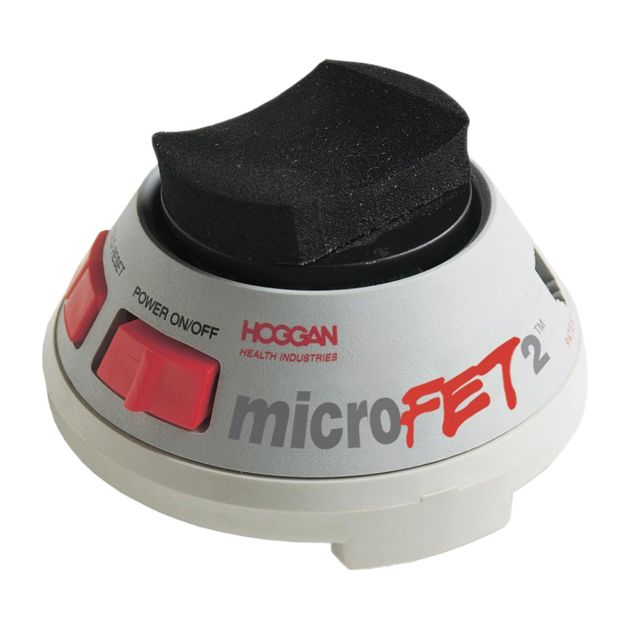
\includegraphics[width=0.45\textwidth]{img/MicroFET 2.jpg}
        \caption{Dispositivo MicroFET 2}
        \label{fig:activforce}
    \end{figure}
    
    \item MAP 80K1S: Es un dispositivo portátil e inalámbrico creado por la empresa alemana KERN \& SOHN. Es un dinamómetro de mano utilizado específicamente para tratamientos de rehabilitación, para la determinación de la fuerza de cierre de mano.
    Presenta cuatro modos de medición: tiempo real, valor máximo. valor promedio y de contaje. 
    Es utilizado en sesiones de rehabilitación para detectar la disminución de fuerza y la evolución del paciente entre sesiones. Cuenta con una pantalla digital donde se puede observar las mediciones realizadas.
    Es un dispositivo de compra libre cuyo precio ronda los 280€. En la \textit{Figura 3.4} se puede ver una imagen del dispositivo.
      \begin{figure}[h]
        \centering
        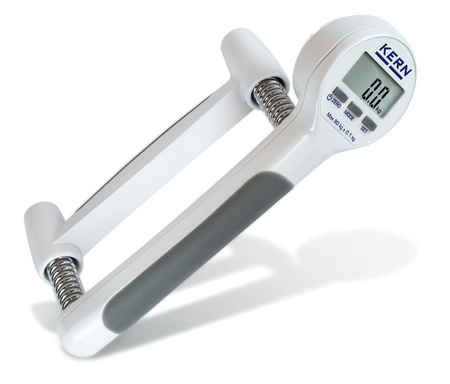
\includegraphics[width=0.5\textwidth]{img/MAP-80K1S.jpg}
        \caption{Dispositivo MAP 80K1S}
        \label{fig:activforce}
    \end{figure}
    
    \item Squeezy dynamometer: Es un dispositivo portátil, un dinamómetro de presión hidráulica de mano cuya medición se realiza apretando la perilla, generando presión que se transfiere al calibrador, el cual muestra con precisión la fuerza ejercida. Es un dispositivo de compra libre cuyo precio ronda los 70 €. En la \textit{Figura 3.5} se puede ver una imagen del dispositivo.
    
     \begin{figure}[h]
        \centering
        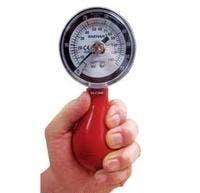
\includegraphics[width=0.5\textwidth]{img/Dinamometro pera.jpeg}
        \caption{Dinamometro de Pera}
        \label{fig:activforce}
    \end{figure}
\end{itemize}
\subsection{Artículos relacionados:}
